\documentclass{article}
\usepackage[utf8]{inputenc}
\usepackage[top=1in]{geometry}
\usepackage{graphicx}
\usepackage{booktabs}
\usepackage{amsmath,amssymb}
\usepackage{xcolor}
\usepackage{multirow}
\usepackage{tikz}
\usetikzlibrary{matrix,shapes,arrows,fit,tikzmark}

% Calligraphic fonts
\newcommand{\calA}{{\cal A}}
\newcommand{\calB}{{\cal B}}
\newcommand{\calC}{{\cal C}}
\newcommand{\calD}{{\cal D}}
\newcommand{\calE}{{\cal E}}
\newcommand{\calF}{{\cal F}}
\newcommand{\calG}{{\cal G}}
\newcommand{\calH}{{\cal H}}
\newcommand{\calI}{{\cal I}}
\newcommand{\calJ}{{\cal J}}
\newcommand{\calK}{{\cal K}}
\newcommand{\calL}{{\cal L}}
\newcommand{\calM}{{\cal M}}
\newcommand{\calN}{{\cal N}}
\newcommand{\calO}{{\cal O}}
\newcommand{\calP}{{\cal P}}
\newcommand{\calQ}{{\cal Q}}
\newcommand{\calR}{{\cal R}}
\newcommand{\calS}{{\cal S}}
\newcommand{\calT}{{\cal T}}
\newcommand{\calU}{{\cal U}}
\newcommand{\calV}{{\cal V}}
\newcommand{\calW}{{\cal W}}
\newcommand{\calX}{{\cal X}}
\newcommand{\calY}{{\cal Y}}
\newcommand{\calZ}{{\cal Z}}

% Sets:
\newcommand{\setA}{\textsf{A}}
\newcommand{\setB}{\textsf{B}}
\newcommand{\setC}{\textsf{C}}
\newcommand{\setD}{\textsf{D}}
\newcommand{\setE}{\textsf{E}}
\newcommand{\setF}{\textsf{F}}
\newcommand{\setG}{\textsf{G}}
\newcommand{\setH}{\textsf{H}}
\newcommand{\setI}{\textsf{I}}
\newcommand{\setJ}{\textsf{J}}
\newcommand{\setK}{\textsf{K}}
\newcommand{\setL}{\textsf{L}}
\newcommand{\setM}{\textsf{M}}
\newcommand{\setN}{\textsf{N}}
\newcommand{\setO}{\textsf{O}}
\newcommand{\setP}{\textsf{P}}
\newcommand{\setQ}{\textsf{Q}}
\newcommand{\setR}{\textsf{R}}
\newcommand{\setS}{\textsf{S}}
\newcommand{\setT}{\textsf{T}}
\newcommand{\setU}{\textsf{U}}
\newcommand{\setV}{\textsf{V}}
\newcommand{\setW}{\textsf{W}}
\newcommand{\setX}{\textsf{X}}
\newcommand{\setY}{\textsf{Y}}
\newcommand{\setZ}{\textsf{Z}}

% Vectors
\newcommand{\bfa}{\mathbf{a}}
\newcommand{\bfb}{\mathbf{b}}
\newcommand{\bfc}{\mathbf{c}}
\newcommand{\bfd}{\mathbf{d}}
\newcommand{\bfe}{\mathbf{e}}
\newcommand{\bff}{\mathbf{f}}
\newcommand{\bfg}{\mathbf{g}}
\newcommand{\bfh}{\mathbf{h}}
\newcommand{\bfi}{\mathbf{i}}
\newcommand{\bfj}{\mathbf{j}}
\newcommand{\bfk}{\mathbf{k}}
\newcommand{\bfl}{\mathbf{l}}
\newcommand{\bfm}{\mathbf{m}}
\newcommand{\bfn}{\mathbf{n}}
\newcommand{\bfo}{\mathbf{o}}
\newcommand{\bfp}{\mathbf{p}}
\newcommand{\bfq}{\mathbf{q}}
\newcommand{\bfr}{\mathbf{r}}
\newcommand{\bfs}{\mathbf{s}}
\newcommand{\bft}{\mathbf{t}}
\newcommand{\bfu}{\mathbf{u}}
\newcommand{\bfv}{\mathbf{v}}
\newcommand{\bfw}{\mathbf{w}}
\newcommand{\bfx}{\mathbf{x}}
\newcommand{\bfy}{\mathbf{y}}
\newcommand{\bfz}{\mathbf{z}}


\newcommand{\bfalpha}{\boldsymbol{\alpha}}
\newcommand{\bfbeta}{\boldsymbol{\beta}}
\newcommand{\bfgamma}{\boldsymbol{\gamma}}
\newcommand{\bfdelta}{\boldsymbol{\delta}}
\newcommand{\bfepsilon}{\boldsymbol{\epsilon}}
\newcommand{\bfzeta}{\boldsymbol{\zeta}}
\newcommand{\bfeta}{\boldsymbol{\eta}}
\newcommand{\bftheta}{\boldsymbol{\theta}}
\newcommand{\bfiota}{\boldsymbol{\iota}}
\newcommand{\bfkappa}{\boldsymbol{\kappa}}
\newcommand{\bflambda}{\boldsymbol{\lambda}}
\newcommand{\bfmu}{\boldsymbol{\mu}}
\newcommand{\bfnu}{\boldsymbol{\nu}}
\newcommand{\bfomicron}{\boldsymbol{\omicron}}
\newcommand{\bfpi}{\boldsymbol{\pi}}
\newcommand{\bfrho}{\boldsymbol{\rho}}
\newcommand{\bfsigma}{\boldsymbol{\sigma}}
\newcommand{\bftau}{\boldsymbol{\tau}}
\newcommand{\bfupsilon}{\boldsymbol{\upsilon}}
\newcommand{\bfphi}{\boldsymbol{\phi}}
\newcommand{\bfchi}{\boldsymbol{\chi}}
\newcommand{\bfpsi}{\boldsymbol{\psi}}
\newcommand{\bfomega}{\boldsymbol{\omega}}
\newcommand{\bfxi}{\boldsymbol{\xi}}
\newcommand{\bfell}{\boldsymbol{\ell}}

% Matrices
\newcommand{\bfA}{\mathbf{A}}
\newcommand{\bfB}{\mathbf{B}}
\newcommand{\bfC}{\mathbf{C}}
\newcommand{\bfD}{\mathbf{D}}
\newcommand{\bfE}{\mathbf{E}}
\newcommand{\bfF}{\mathbf{F}}
\newcommand{\bfG}{\mathbf{G}}
\newcommand{\bfH}{\mathbf{H}}
\newcommand{\bfI}{\mathbf{I}}
\newcommand{\bfJ}{\mathbf{J}}
\newcommand{\bfK}{\mathbf{K}}
\newcommand{\bfL}{\mathbf{L}}
\newcommand{\bfM}{\mathbf{M}}
\newcommand{\bfN}{\mathbf{N}}
\newcommand{\bfO}{\mathbf{O}}
\newcommand{\bfP}{\mathbf{P}}
\newcommand{\bfQ}{\mathbf{Q}}
\newcommand{\bfR}{\mathbf{R}}
\newcommand{\bfS}{\mathbf{S}}
\newcommand{\bfT}{\mathbf{T}}
\newcommand{\bfU}{\mathbf{U}}
\newcommand{\bfV}{\mathbf{V}}
\newcommand{\bfW}{\mathbf{W}}
\newcommand{\bfX}{\mathbf{X}}
\newcommand{\bfY}{\mathbf{Y}}
\newcommand{\bfZ}{\mathbf{Z}}


\newcommand{\bfGamma}{\boldsymbol{\Gamma}}
\newcommand{\bfDelta}{\boldsymbol{\Delta}}
\newcommand{\bfTheta}{\boldsymbol{\Theta}}
\newcommand{\bfLambda}{\boldsymbol{\Lambda}}
\newcommand{\bfPi}{\boldsymbol{\Pi}}
\newcommand{\bfSigma}{\boldsymbol{\Sigma}}
\newcommand{\bfUpsilon}{\boldsymbol{\Upsilon}}
\newcommand{\bfPhi}{\boldsymbol{\Phi}}
\newcommand{\bfPsi}{\boldsymbol{\Psi}}
\newcommand{\bfOmega}{\boldsymbol{\Omega}}


% Blackboard Bold:
\newcommand{\bbA}{\mathbb{A}}
\newcommand{\bbB}{\mathbb{B}}
\newcommand{\bbC}{\mathbb{C}}
\newcommand{\bbD}{\mathbb{D}}
\newcommand{\bbE}{\mathbb{E}}
\newcommand{\bbF}{\mathbb{F}}
\newcommand{\bbG}{\mathbb{G}}
\newcommand{\bbH}{\mathbb{H}}
\newcommand{\bbI}{\mathbb{I}}
\newcommand{\bbJ}{\mathbb{J}}
\newcommand{\bbK}{\mathbb{K}}
\newcommand{\bbL}{\mathbb{L}}
\newcommand{\bbM}{\mathbb{M}}
\newcommand{\bbN}{\mathbb{N}}
\newcommand{\bbO}{\mathbb{O}}
\newcommand{\bbP}{\mathbb{P}}
\newcommand{\bbQ}{\mathbb{Q}}
\newcommand{\bbR}{\mathbb{R}}
\newcommand{\bbS}{\mathbb{S}}
\newcommand{\bbT}{\mathbb{T}}
\newcommand{\bbU}{\mathbb{U}}
\newcommand{\bbV}{\mathbb{V}}
\newcommand{\bbW}{\mathbb{W}}
\newcommand{\bbX}{\mathbb{X}}
\newcommand{\bbY}{\mathbb{Y}}
\newcommand{\bbZ}{\mathbb{Z}}




\title{Homework 2  solution}
\author{Max marks: 155}
\newtheorem{prob}{Problem}

\newcommand{\bx}{\bar{x}}
\newcommand{\by}{\bar{y}}
\newcommand{\bz}{\bar{z}}
\newcommand{\bA}{\bar{A}}
\newcommand{\bB}{\bar{B}}
\newcommand{\bC}{\bar{C}}
\newcommand{\cred}{\color{red}}
\newcommand{\cg}{\color{green!60!black}}
\newcommand{\cb}{\color{blue}}
% Some options common to all the nodes and paths
\tikzset{   
  every picture/.style={remember picture,baseline},
  every node/.style={anchor=base,align=center,outer sep=1.5pt},
  every path/.style={thick},
}

\newcommand\marktopleft[1]{%
  \tikz[overlay,remember picture] 
  \node (marker-#1-a) at (.3em,.3em) {};%
}
\newcommand\markbottomright[2]{%
  \tikz[overlay,remember picture] 
  \node (marker-#1-b) at (.1em,.3em) {};%
  \tikz[overlay,remember picture,inner sep=1pt]
  \node[draw={#2},rounded corners,fit=(marker-#1-a.north west) (marker-#1-b.south east)] {};%
}
\newcommand\markpolytopleft[1]{%
  \tikz[overlay,remember picture]%
  \node (marker-#1-tl) at (.3em,.3em) {};%
}
\newcommand\markpolytopright[1]{%
  \tikz[overlay,remember picture]%
  \node (marker-#1-tr) at (.3em,.3em) {};%
}
\newcommand\markpolybottomright[1]{%
  \tikz[overlay,remember picture] 
  \node (marker-#1-br) at (.3em,.3em) {};%
  }
\newcommand\markpolybottomleft[2]{%
  \tikz[overlay,remember picture]
  \node (marker-#1-bl) at (.3em,.3em) {};%
  \tikz[overlay,remember picture,inner sep=1pt]
  \path [draw={#2},rounded corners]
  (marker-#1-tl.north west) --
  (marker-#1-tl.north east) --
  (marker-#1-bl.south east) --
  (marker-#1-br.south west);%
}


\begin{document}


\maketitle

\begin{prob}
  Read Chapter 2 up to Section 2.7 of Harris and Harris textbook. Write a statement saying that you have read and understood the chapter. [5 marks]
\end{prob}

\begin{prob}
If the SOP form for $ \bar{f} = AB\bC+\bA\bB$, then give the POS form for
$f$. [10 marks]
\end{prob}
\subsubsection*{Solution}

Take inverse on both sides
\begin{align*}
  \overline{\bar{f}} &= \overline{AB\bC+\bA\bB} &
  \\
  f  &= \overline{AB\bC} \cdot \overline{\bA\bB} & \text{ by DeMorgan's}
  \\
    &= (\bA + \bB + C) (A + B) & \text{ by DeMorgan's}
\end{align*}

\begin{prob}
Use DeMorgan's Theorem to find $f$  if  $\bar{f} = (A + \bB C)D + EF$. [10 marks]
\end{prob}

\subsubsection*{Solution}
Take inversion on both sides
\begin{align*}
  \overline{\bar{f}} &= \overline{(A+\bB C)D + EF} &
  \\
  f  &= \overline{((A+\bB C)D)} \cdot \overline{EF} & \text{ by DeMorgan's}
  \\
  &= (\overline{(A+\bB C)} + \bar{D}) (\bar{E}+\bar{F}) & \text{ by DeMorgan's}
  \\
  &= (\bA\overline{(\bB C)} + \bar{D}) (\bar{E}+\bar{F}) & \text{ by DeMorgan's}
  \\
  &= (\bA(B + \bC) + \bar{D}) (\bar{E}+\bar{F}) & \text{ by DeMorgan's}
\end{align*}

\begin{table}
  \centering
  \begin{tabular}{c|ccc||c}
    \toprule
    Row & $x_1$ & $x_2$ & $x_3$ & f \\
    \midrule
    0 & 0 & 0 & 0 & 0 \\
    1 & 0 & 0 & 1 & 1 \\
    2 & 0 & 1 & 0 & 1 \\
    3 & 0 & 1 & 1 & 0 \\
    4 & 1 & 0 & 0 & 1 \\
    5 & 1 & 0 & 1 & 0 \\
    6 & 1 & 1 & 0 & 0 \\
    7 & 1 & 1 & 1 & 1 \\
    \bottomrule
    \end{tabular}
    \caption{Truth table for a 3-way light switch}
    \label{tab:3-way-light-switch}
\end{table}

\begin{prob}
  For the function $f = AB\bC + BD$,
  \begin{enumerate}
    \item Write the Truth table. [10 marks]
    \item Write $f$ in Sum of Products form. [10 marks]
    \item Write $f$ in canonical minterm form. [10 marks]
    \item Write $f$ as Product of Sums. [10 marks]
    \item Write $f$ in canonical maxterm form. [10 marks]
  \end{enumerate}
\end{prob}

\begin{prob}
 Implement the function in Table~\ref{tab:3-way-light-switch} using only NAND
 gates. [10 marks]
\end{prob}
\subsubsection*{Solution}
To implement the function using NAND gates, we seek the SOP form of the
function,
\\
\begin{tabular}{c|c|c|c|c}
  \toprule
  & \multicolumn{2}{c|}{$\bx_1$} & \multicolumn{2}{c}{$x_1$}
  \\
  & $\bx_2$ & \multicolumn{2}{c|}{$x_2$} & $\bx_2$
  \\ \midrule
  $\bx_3$
  & 0 & 1 & 0 & 1
  \\
  $x_3$
  & 1 & 0 & 1 & 0
  \\\bottomrule
\end{tabular}.
\\
The function cannot be simplified beyond minterms.
\begin{align*}
  f &= \bx_1 \bx_2 x_3 + \bx_1 x_2 \bx_3 + x_1 \bx_2 \bx_3 + x_1 x_2 x_3
  \\
    &= \overline{\overline{\bx_1 \bx_2 x_3}} + \overline{\overline{\bx_1 x_2 \bx_3}} + \overline{\overline{x_1 \bx_2 \bx_3}} + \overline{\overline{x_1 x_2 x_3}}
  \\
    &= \overline{\overline{\bx_1 \bx_2 x_3} \cdot {\overline{\bx_1 x_2 \bx_3}} \cdot {\overline{x_1 \bx_2 \bx_3}} \cdot {\overline{x_1 x_2 x_3}}}
\end{align*}
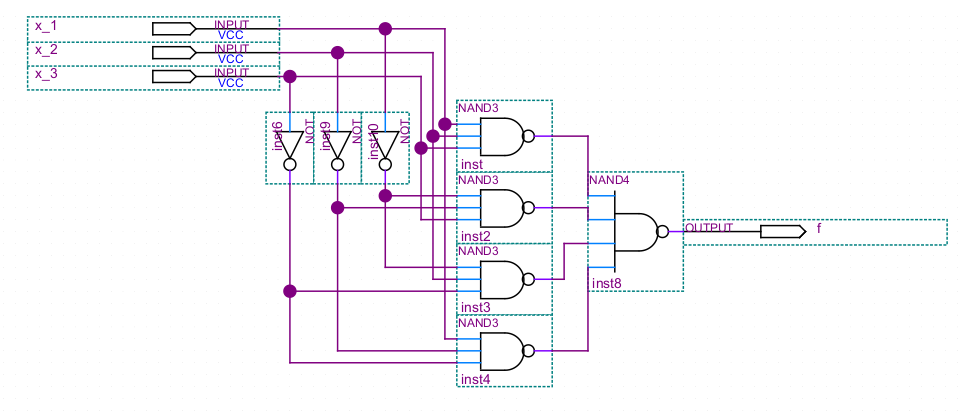
\includegraphics[width=\linewidth]{files/hw2p3.png}

\begin{prob}
 Implement the function in Table~\ref{tab:3-way-light-switch} using only NOR
 gates. [10 marks]
\end{prob}
\subsubsection*{Solution}
To implement the function using NAND gates, we seek the POS form of the
function. We plot the K-map for $\bar{f}$,
\\
\begin{tabular}{c|c|c|c|c}
  \toprule
  & \multicolumn{2}{c|}{$\bx_1$} & \multicolumn{2}{c}{$x_1$}
  \\
  & $\bx_2$ & \multicolumn{2}{c|}{$x_2$} & $\bx_2$
  \\ \midrule
  $\bx_3$
  & 1 & 0 & 1 & 0
  \\
  $x_3$
  & 0 & 1 & 0 & 1
  \\\bottomrule
\end{tabular}.
\\
The function $\bar{f}$ cannot be simplified further,
\[
  \bar{f} = \bx_1 \bx_2 \bx_3  + \bx_1 \bx_2 x_3  + \bx_1 x_2 \bx_3 + x_1 \bx_2 x_3
\]
Taking inverse of both sides and observing $\overline{\bar{f}} = f$.
{\tiny
\begin{align*}
  f &= (x_1 + x_2 + x_3)(x_1 + \bx_2 + \bx_3)(\bx_1 + x_2 + \bx_3)(\bx_1 + \bx_2 + x_3)
      \\
    &=\overline{\overline{(x_1 + x_2 + x_3)}}\overline{\overline{(x_1 + \bx_2 + \bx_3)}}\overline{\overline{(\bx_1 + x_2 + \bx_3)}}\overline{\overline{(\bx_1 + \bx_2 + x_3)}}
      \end{align*}
}{\tiny
\begin{align*}
  &=\overline{\overline{{(x_1 + x_2 + x_3)}} + {\overline{(x_1 + \bx_2 + \bx_3)}}
  + {\overline{(\bx_1 + x_2 + \bx_3)}} + {\overline{(\bx_1 + \bx_2 + x_3)}}}
\end{align*}
}
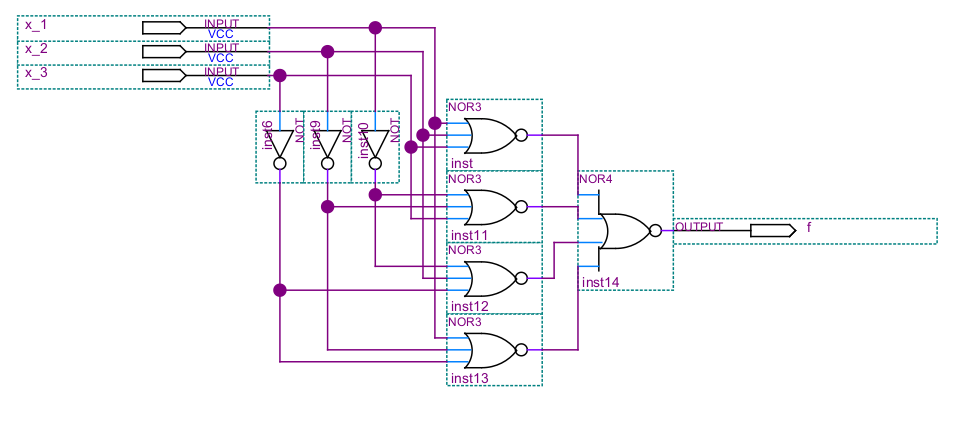
\includegraphics[width=\linewidth]{files/hw2p4.png}


\begin{prob}
Find the minimum-cost SOP and POS forms for the function $f(x_1 , x_2 , x_3 ) =
m(1, 3, 4, 5)$. \cite[Prob 2.37]{brown2013fundamentals} [10 marks]
\label{prob:237}
\end{prob}

\subsubsection*{Solution}

Minimum cost SOP
\\
\begin{tabular}{c|c|c|c|c}
  \toprule
  & \multicolumn{2}{c|}{$\bx_1$} & \multicolumn{2}{c}{$x_1$}
  \\
  & $\bx_2$ & \multicolumn{2}{c|}{$x_2$} & $\bx_2$
  \\ \midrule
  $\bx_3$
  & 0 & 0 & 0 & {\color{red}1}
  \\
  $x_3$
  & {\color{green}1} & {\color{green}1} & 0 & {\color{red}1}
  \\\bottomrule
\end{tabular}.
\\
\begin{align}
  f = {\cred x_1 \bx_2} + {\cg \bx_1 x_3}
\end{align}
Cost = 2 AND  + 1 OR + (2 * (2 input per AND gates) + 2 input per OR gate) inputs = 9

To find Minimum cost POS, we draw K-map for $\bar{f}$.
\\
\begin{tabular}{c|c|c|c|c}
  \toprule
  & \multicolumn{2}{c|}{$\bx_1$} & \multicolumn{2}{c}{$x_1$}
  \\
  & $\bx_2$ & \multicolumn{2}{c|}{$x_2$} & $\bx_2$
  \\ \midrule
  $\bx_3$
  & \cred 1 & \cred 1 & \cg 1 & 0
  \\
  $x_3$
  & 0 & 0 & \cg 1 & 0
  \\\bottomrule
\end{tabular}.
\\
\begin{align}
  \bar{f} &= {\cred \bx_1 \bx_3} + {\cg x_1 x_2 }
  \\
  \implies f &= {\cred (x_1 + x_3)}{\cg (\bx_1 + \bx_2) }
\end{align}
Cost = 2 OR + 1 AND + (2 * (2 inputs per OR gate) + 2 input AND gate) inputs = 9

\begin{prob}
Find the minimum-cost SOP and POS forms for the function $f(x_1 , x_2 , x_3) =
\sum m(1, 5, 7) + D(2, 4)$. \cite[Prob 2.38]{brown2013fundamentals} [10 marks]
\end{prob}

\subsubsection*{Solution}

Minimum cost SOP
\\
\begin{tabular}{c|c|c|c|c}
  \toprule
  & \multicolumn{2}{c|}{$\bx_1$} & \multicolumn{2}{c}{$x_1$}
  \\
  & $\bx_2$ & \multicolumn{2}{c|}{$x_2$} & $\bx_2$
  \\ \midrule
  $\bx_3$
                                  & 0 & d & 0 & d
  \\
  $x_3$
                                  & \cb 1 & 0 & {\cg 1} & {\cg 1} + {\cb 1}
  \\\bottomrule
\end{tabular}.
\\
\begin{align}
  f = {\cred x_1 \bx_2} + {\cb \bx_2 x_3}
\end{align}
Cost = 3 AND  + 1 OR + (2 * (2 input per AND gate) + 3 inputs per OR gate) inputs = 10

To find minimum cost POS, we draw K-map for $\bar{f}$,
\\
\begin{tabular}{c|c|c|c|c}
  \toprule
  & \multicolumn{2}{c|}{$\bx_1$} & \multicolumn{2}{c}{$x_1$}
  \\
  & $\bx_2$ & \multicolumn{2}{c|}{$x_2$} & $\bx_2$
  \\ \midrule
  $\bx_3$
  & \cred 1 & \cred d  + \cg d + \cb d & \cb 1 & d
  \\
  $x_3$
  & 0 & \cg 1 & 0 & 0
  \\\bottomrule
\end{tabular}.
\\
\begin{align}
  \bar{f} &= {\cred \bx_1 \bx_3 } + {\cg \bx_1 x_2 } + {\cb x_2 \bx_3}
  \\
  \implies f &= {\cred (x_1 + x_3)}{\cg (x_1 + \bx_2) } {\cb (\bx_2 + x_3)}
\end{align}
Cost = 3 OR + 1 AND + (3*(2 inputs per OR gate)+3 inputs per AND gate) inputs = 13

\begin{prob}
Find the minimum-cost SOP and POS forms for the function $f(x_1 , x_2 , x_3,
x_4) = \prod M(1, 2, 4, 5, 7, 8, 9, 10, 12, 14, 15).$ \cite[Prob
2.39]{brown2013fundamentals} [10 marks]
\end{prob}

\subsubsection*{Solution}

The function $f$ is zero at the maxterms. We draw the following K-map,
\\
\begin{tabular}{c|c|c|c|c|c}
  \toprule
  && \multicolumn{2}{c|}{$\bx_1$} & \multicolumn{2}{c}{$x_1$}
  \\
  && $\bx_2$ & \multicolumn{2}{c|}{$x_2$} & $\bx_2$
  \\ \midrule
  \multirow{2}{*}{$\bx_3$} & $\bx_4$
                                  & 1 & 0 & 0 & 0
  \\
  & $x_4$
                                  & 0 & 0 & 1 & 0
  \\
  \multirow{2}{*}{$x_3$}   &  $x_4$
                                  & \cred 1 & 0 & 0 & \cred 1
  \\
  & $\bx_4$
                                  & 0 & 1 & 0 & 0
  \\\bottomrule
\end{tabular}.
\\
\begin{align}
  f = \bx_1 \bx_2 \bx_3 \bx_4 + {\cred \bx_2 x_3 x_4} + \bx_1 x_2  x_3 \bx_4 + x_1 x_2 \bx_3 x_4
\end{align}
Cost = 4 AND gates + 1 OR gate + (4+3+4+4 inputs to the AND gates + 3 inputs to the OR
gate) = 23.

To find the POS form, we draw K-map for $\bar{f}$,
\\
\begin{tabular}{c|c|c|c|c|c}
  \toprule
  && \multicolumn{2}{c|}{$\bx_1$} & \multicolumn{2}{c}{$x_1$}
  \\
  && $\bx_2$ & \multicolumn{2}{c|}{$x_2$} & $\bx_2$
  \\ \midrule
  \multirow{2}{*}{$\bx_3$} & $\bx_4$
                           & 0 & \cred 1 & \color{purple} 1 & \color{purple} 1
  \\
  & $x_4$
                                  & \cb 1 & \cred 1 & 0 & \cb 1
  \\
  \multirow{2}{*}{$x_3$}   &  $x_4$
                                  & 0 & \color{cyan} 1 & \color{cyan} 1 & 0
  \\
  & $\bx_4$
                                  & \color{yellow} 1 & 0 & \color{purple} 1 & \color{purple} 1 + \color{yellow} 1
  \\\bottomrule
\end{tabular}.
\\
\begin{align*}
  \bar{f} &= \cred \bx_1 x_2 \bx_3 + \color{cyan} x_2 x_3 x_4 
  + \cb \bx_2 \bx_3 x_4 + \color{purple} x_1 \bx_4 + \color{yellow} \bx_2 x_3 \bx_4
  \\
  \implies &f = {\cred (x_1 + \bx_2 + x_3)}{\color{cyan} (\bx_2 + \bx_3 + \bx_4)}
  {\cb (x_2 + x_3 + \bx_4)} {\color{purple} (\bx_1 + x_4)}{\color{yellow}(x_2 + \bx_3 + x_4)}
\end{align*}

\begin{prob}
Find the minimum-cost SOP and POS forms for the function $f(x_1 , x_2 , x_3, x_4) =
\sum m(2, 8, 9, 12, 15) + D(1, 3, 6, 7).$ \cite[Prob
2.40]{brown2013fundamentals} [10 marks]
\end{prob}

\subsubsection*{Solution}

The K-map for $f$ is
\\
\begin{tabular}{c|c|c|c|c|c}
  \toprule
  && \multicolumn{2}{c|}{$\bx_1$} & \multicolumn{2}{c}{$x_1$}
  \\
  && $\bx_2$ & \multicolumn{2}{c|}{$x_2$} & $\bx_2$
  \\ \midrule
  \multirow{2}{*}{$\bx_3$} & $\bx_4$
                                  & 0 & 0 & \cg 1 & \cg 1 + \cb 1
  \\
  & $x_4$
                                  & d & 0 & 0 & \cb 1
  \\
  \multirow{2}{*}{$x_3$}   &  $x_4$
                                  & \cred d & \color{cyan} d & \color{cyan} 1 & 0
  \\
  & $\bx_4$
                                  & \cred 1 & d & 0 & 0
  \\\bottomrule
\end{tabular}.
\\
\[ f = { \cred \bx_1 \bx_2 x_3} +  { \cg x_1 \bx_3 \bx_4 } + {\cb x_1 \bx_2 \bx_3 }
  + { \color{cyan} x_2 x_3 x_4 }
\]
  Cost = 4 AND gates + 1 OR gate + (3 + 3 + 3 +3 inputs to the AND gates + 4
  inputs to the OR gate) = 21
  \\
The K-map for $\bar{f}$ is
\\
\begin{tabular}{c|c|c|c|c|c}
  \toprule
  && \multicolumn{2}{c|}{$\bx_1$} & \multicolumn{2}{c}{$x_1$}
  \\
  && $\bx_2$ & \multicolumn{2}{c|}{$x_2$} & $\bx_2$
  \\ \midrule
  \multirow{2}{*}{$\bx_3$} & $\bx_4$
                                  & \cred 1 & \cred 1 & 0 & 0
  \\
  & $x_4$
                                  & \cred d & \cred 1 + \cb  1 & \cb 1 & 0
  \\
  \multirow{2}{*}{$x_3$}   &  $x_4$
                                  & d & d & 0 & \color{cyan} 1
  \\
  & $\bx_4$
                                  & 0 & d & \cg 1 & \cg 1 +  \color{cyan} 1
  \\\bottomrule
\end{tabular}
\\
\begin{align}
  \bar{f} &= { \cred \bx_1 \bx_3 }  +  { \cb  x_2 \bx_3 x_4 }+  {\cg x_1 x_3 \bx_4
  } + { \color{cyan} x_1 \bx_2 x_3}.
  \\
  \implies &f = { \cred (x_1 + x_3) } {\cb (\bx_2 + x_3 + \bx_4) }
  \notag\\
  &\qquad {\cg (\bx_1 + \bx_3 + x_4) }
  {\color{cyan} (\bx_1 + x_2 + \bx_3 )}.
\end{align}
Cost = 4 OR gates + 1 AND gate + (2 + 3 + 3 + 3 inputs to OR gates and 4 inputs
to the AND gate) = 20 



\begin{prob}
Derive a minimum-cost realization of the four-variable function that is equal to 1 if exactly
two or exactly three of its variables are equal to 1; otherwise it is equal to
0. \cite[Prob 2.46]{brown2013fundamentals} [10 marks]
\end{prob}

\subsubsection*{Solution}

\begin{tabular}{c|cccc||c|r}
  \toprule
  Row & $x_1$  & $x_2$ & $x_3$ & $x_4$ & f & Reason\\
  \midrule
   0 & 0 & 0 &  0 & 0 & 0 & 
   \\
   1 & 0 & 0 &  0 & 1 & 0 &
   \\
   2 & 0 & 0 &  1 & 0 & 0 &
   \\
   3 & 0 & 0 &  1 & 1 & 1 & 2-var are one
   \\
   4 & 0 & 1 &  0 & 0 & 0 & 
   \\
   5 & 0 & 1 &  0 & 1 & 1 & 2-var
   \\
   6 & 0 & 1 &  1 & 0 & 1 & 2-var
   \\
   7 & 0 & 1 &  1 & 1 & 1 & 3-var
   \\
   8 & 1 & 0 &  0 & 0 & 0 & 
   \\
   9 & 1 & 0 &  0 & 1 & 1 & 2-var
  \\
  10 & 1 & 0 &  1 & 0 & 1 & 2-var
  \\
  11 & 1 & 0 &  1 & 1 & 1 & 3-var
  \\
  12 & 1 & 1 &  0 & 0 & 1 & 2-var
  \\
  13 & 1 & 1 &  0 & 1 & 1 & 3-var
  \\
  14 & 1 & 1 &  1 & 0 & 1 & 3-var
  \\
  15 & 1 & 1 &  1 & 1 & 0 &
  \\
  \bottomrule
\end{tabular}

K-map for the function $f$ is
\\
\begin{tabular}{c|c|c|c|c|c}
  \toprule
  && \multicolumn{2}{c|}{$\bx_1$} & \multicolumn{2}{c}{$x_1$}
  \\
  && $\bx_2$ & \multicolumn{2}{c|}{$x_2$} & $\bx_2$
  \\ \midrule
  \multirow{2}{*}{$\bx_3$} & $\bx_4$
                                  & 0 & 0 &  \color{yellow} 1 & 0
  \\
  & $x_4$
                                  & 0 & \cred 1 & \cred 1 + \color{yellow} 1 & \cb 1
  \\
  \multirow{2}{*}{$x_3$}   &  $x_4$
                                  & \color{cyan} 1 & \color{cyan} 1 & 0 & \cb 1
  \\
  & $\bx_4$
                                  & 0 & \cg 1 & \cg 1 + \color{orange} 1 & \color{orange} 1
  \\\bottomrule
\end{tabular}.
\\
\begin{align*}
f &= { \cred x_2 \bx_3 x_4 } +  { \cg x_2 x_3 \bx_4} + {\cb x_1 \bx_2 x_4} +
  {\color{cyan} \bx_1 x_3 x_4 }
  \\
  &\qquad + {\color{orange} x_1 x_3 \bx_4} +
{\color{yellow} x_1 x_2 \bx_3 }
  \end{align*}
 Cost = 5 AND gates + 1 OR gate + (5*3 inputs per AND gate + 5 inputs to the OR
 gate) = 26

 K-map for the inverted function $\bar{f}$ is
 \\
 \begin{tabular}{c|c|c|c|c|c}
   \toprule
   && \multicolumn{2}{c|}{$\bx_1$} & \multicolumn{2}{c}{$x_1$}
   \\
   && $\bx_2$ & \multicolumn{2}{c|}{$x_2$} & $\bx_2$
   \\ \midrule
   \multirow{2}{*}{$\bx_3$} & $\bx_4$
                                   & \cred 1 + \cg 1 + \cb 1 + \color{cyan} 1 & \cred 1 &  0 &  \cg 1
   \\
   & $x_4$
                                   & \cb 1 & 0 & 0 & 0
   \\
   \multirow{2}{*}{$x_3$}   &  $x_4$
                                   & 0 & 0 & 1 & 0
   \\
   & $\bx_4$
                                   & \color{cyan} 1 & 0 & 0 & 0
   \\\bottomrule
 \end{tabular}.
 \\
 \begin{align*}
   \bar{f} &= {\cred \bx_1 \bx_3 \bx_4 } + {\cg \bx_2 \bx_3 \bx_4} + {\cb \bx_1 \bx_2 \bx_3 }
   \\
   &\qquad + {\color{cyan} \bx_1 \bx_2 \bx_4 } + x_1 x_2 x_3 x_4
   \\
   f &= {\cred (x_1 + x_3 + x_4) } {\cg (x_2 + x_3 + x_4)} 
   \\
           &\qquad {\cb (x_1 + x_2 + x_3)}{\color{cyan} (x_1 + x_2 + x_4)}
   \\
   &\qquad (\bx_1 + \bx_2+ \bx_3 + \bx_4)
 \end{align*}
 Cost = 5 OR gates + 1 AND gate + (4 * 3 inputs per OR gate + 4 inputs to one OR
 gate + 5 inputs to 1 AND gate = 27

 The minimal cost representation is the SOP representation:
 \begin{align*}
   f &= { \cred x_2 \bx_3 x_4 } +  { \cg x_2 x_3 \bx_4} + {\cb x_1 \bx_2 x_4} +
       {\color{cyan} \bx_1 x_3 x_4 }
   \\
     &\qquad + {\color{orange} x_1 x_3 \bx_4} +
       {\color{yellow} x_1 x_2 \bx_3 }
 \end{align*}


\begin{prob}
  Find the minimum-cost SOP and POS forms for the function \\
  $f(x_1 , \dots, x_5) =
  \sum m(1, 3, 4, 6, 8, 9, 11, 13, 14, 16, 19, 20, 21, 22, 24, 25) + D(5, 7,
  12, 15, 17, 23).$  \cite[Prob 2.42]{brown2013fundamentals} [10 marks]
  \label{prob:prob10}
\end{prob}

\subsubsection*{Solution}

\begin{table*}[h]
  \centering
  \begin{tabular}{c|c|cccccccc}
  \toprule
  && \multicolumn{4}{c|}{$\bx_1$} & \multicolumn{4}{c}{$x_1$}
    \\
    && \multicolumn{2}{c|}{$\bx_2$} & \multicolumn{2}{c|}{$x_2$}
               & \multicolumn{2}{c|}{$\bx_2$} & \multicolumn{2}{c}{$x_2$}
  \\
  && $\bx_3$ & \multicolumn{2}{|c|}{$x_3$} & $\bx_3$
              & $\bx_3$ & \multicolumn{2}{|c|}{$x_3$} & $\bx_3$
  \\ \midrule
  \multirow{2}{*}{$\bx_4$} & $\bx_5$ &
                                       0 & \marktopleft{g1} 1 & \marktopleft{c2} d & \marktopleft{b2} 1
                                         &  \marktopleft{p1} \color{purple} 1 & \marktopleft{c1} 1 &  0 &  \marktopleft{b4}\cb 1
    \\
    & $x_5$ &
              \marktopleft{r1} \marktopleft{o1}
              1  & d   & 1 & 1 \markbottomright{b2}{blue} 
                 & \marktopleft{o2} d   & 1 \markbottomright{p1}{purple}&  0 &\cb 1\markbottomright{b4}{blue}
  \\
    \multirow{2}{*}{$x_4$}   &  $x_5$ &
                                        1 & d \markbottomright{o1}{orange} & d  & \cred 1 
                                                    \markbottomright{r1}{red}
                                              & \color{orange} 1 & d \markbottomright{o2}{orange} &  0 & 0
  \\
    & $\bx_5$ &
                0 & \cg 1 & 1 \markbottomright{c2}{cyan} \markbottomright{g1}{green} & 0
                                              & 0 & \color{cyan} 1 \markbottomright{c1}{cyan} &  0 & 0
  \\\bottomrule
  \end{tabular}\hfill
  % \begin{tabular}{c|c|cc|cc|cc|cc}
  % \toprule
  % && \multicolumn{8}{c}{$x_1 = 0/1$}
  %   \\
  %   && \multicolumn{4}{c|}{$\bx_2$} & \multicolumn{4}{c}{$x_2$}
  % \\
  %   && \multicolumn{2}{c}{$\bx_3$} & \multicolumn{4}{|c|}{$x_3$} & \multicolumn{2}{c}{$\bx_3$}
  % \\ \midrule
  %   \multirow{4}{*}{$\bx_4$} & \multirow{2}{*}{$\bx_5$}
  %   &
  %     \markpolytopleft{b211}1 && 1 && d && 1 
  %   \\
  %   &&& 1  \markpolytopright{b211} && 1 && 0 && 1
  %   \\\cmidrule{2-10}
  %   & \multirow{4}{*}{$x_5$}
  %   &
  %     \markpolybottomleft{b211}{blue} \marktopleft{r211}1 && d && 1 && 1 
  %   \\
  %   &&& d \markpolybottomright{b211} && 1 && 0 && 1
  %   \\\cmidrule{1-1}\cmidrule{3-10}
  %   \multirow{4}{*}{$x_4$}   &  
  %   &
  %     1 && d && d && 1\markbottomright{r211}{red} 
  %   \\
  %   &&& 1 && d && 0 && 0
  %   \\\cmidrule{2-10}
  %   & \multirow{2}*{$\bx_5$}
  %   &
  %     0 && 1 && 1 && 0 
  %   \\
  %   &&& 0 && 1 && 0 && 0
  % \\\bottomrule
  % \end{tabular}\hfill
  
  \caption{K-map for $f$ in problem ~\ref{prob:prob10}. The essential minterm for the Essential
  Prime implicant is indicated with the same color.}
\label{tab:prob10}
\end{table*}

The K-map for the function is in Table~\ref{tab:prob10}.
\[
  f = {\cred \bx_1 x_5 } + {\cg \bx_1 x_3 } + {\color{cyan} x_2 x_3 }
  + {\cb x_2 \bx_3 \bx_4} + {\color{orange} \bx_2 x_5} 
  + {\color{purple} x_1 \bx_2 \bx_4}
\]
 Cost = 6 AND gates + 1 OR gate + (4*2+2*3 inputs per AND gate + 6 inputs to one OR gate) = 27

 The K-map for the function inverse is given in Table~\ref{tab:prob10inv}
 \begin{align*}
   \bar{f} &= {\color{purple} \bx_1 \bx_2 \bx_3 \bx_5} + {\cred x_1 x_2 x_3} + {\cb \bx_3 x_4 \bx_5 } + {\cg x_1 x_2 x_4}
   \\
   \implies  &f = {\color{purple} (x_1 + x_2 + x_3 + x_5)}{\cred (\bx_1 + \bx_2 + \bx_3)}{\cb (x_3 + \bx_4 + x_5)}
               \\&\qquad{\cg (\bx_1 + \bx_2 + \bx_4)}
 \end{align*}
 Cost = 4 OR gate + 1 AND gate + (3*3+4*1 inputs to the OR gates and 4 inputs to the AND gate)=22.
 


\begin{table*}
  \centering
  \begin{tabular}{c|c|cccccccc}
  \toprule
  && \multicolumn{4}{c|}{$\bx_1$} & \multicolumn{4}{c}{$x_1$}
    \\
    && \multicolumn{2}{c|}{$\bx_2$} & \multicolumn{2}{c|}{$x_2$}
               & \multicolumn{2}{c|}{$\bx_2$} & \multicolumn{2}{c}{$x_2$}
  \\
  && $\bx_3$ & \multicolumn{2}{|c|}{$x_3$} & $\bx_3$
              & $\bx_3$ & \multicolumn{2}{|c|}{$x_3$} & $\bx_3$
  \\ \midrule
  \multirow{2}{*}{$\bx_4$} & $\bx_5$
                           & \marktopleft{p1}\color{purple} 1 \markbottomright{p1}{purple} & 0 & d & 0
                                              & 0 & 0 &  \marktopleft{r1}\cred 1 & 0
  \\
  & $x_5$
                                  & 0 & d  & 0 & 0
                                              & d & 0 &  \cred 1 & 0
  \\
  \multirow{2}{*}{$x_4$}   &  $x_5$
                                  & 0 & d & d & 0
                                              & 0 & d  &  \marktopleft{g1}1 &\cg 1
  \\
  & $\bx_5$
  & \marktopleft{p2} \marktopleft{b2} \cb 1 \markbottomright{b2}{blue} \markbottomright{p2}{purple} & 0 & 0 & \marktopleft{b3} \cb 1 \markbottomright{b3}{blue} 
                                              & \marktopleft{b4} \cb 1 \markbottomright{b4}{blue} & 0 &  1 \markbottomright{r1}{red} & \marktopleft{b1} 1 \markbottomright{b1}{blue} \markbottomright{g1}{green}
  \\\bottomrule
  \end{tabular}
  \hfill
%   \begin{tabular}{c|c|cccc}
%   \toprule
%   && \multicolumn{4}{c}{$x_1 = 0/1$}
%     \\
%     && \multicolumn{2}{c|}{$\bx_2$} & \multicolumn{2}{c}{$x_2$}
%                
%   \\
%   && $\bx_3$ & \multicolumn{2}{|c|}{$x_3$} & $\bx_3$
%   \\ \midrule
%   \multirow{2}{*}{$\bx_4$} & $\bx_5$
%                                   & 0/0 & 0/0 & d/\marktopleft{r21}\cred 1 & 0/0
%   \\
%   & $x_5$
%                                   & 0/d & d/0  & 0/\cred 1 & 0/0
%   \\
%   \multirow{2}{*}{$x_4$}   &  $x_5$
%                                   & 0/0 & d/d & d/\marktopleft{g31}1 & 0/\cg 1
%   \\
%   & $\bx_5$
%                                   & \marktopleft{b32}\cb 1/1\markbottomright{b32}{blue} & 0/0 & 0/1\markbottomright{r21}{red} & \marktopleft{b31}{\cb 1}/1\markbottomright{b31}{blue}\markbottomright{g31}{green}
%   \\\bottomrule
% \end{tabular}
  \caption{5-var K-map for $\bar{f}$ in problem ~\ref{prob:prob10}. The
  essential minterms for Essential Prime Implicants (EPI) is shown in the same color.}
\label{tab:prob10inv}
\end{table*}
\bibliography{main}
\bibliographystyle{plain}

\begin{table*}
  \begin{tabular}{c|c|c|c|c|c|c|c|c|c}
  \toprule
  && \multicolumn{4}{c|}{$\bx_1$} & \multicolumn{4}{c}{$x_1$}
    \\
    && \multicolumn{2}{c|}{$\bx_2$} & \multicolumn{2}{c|}{$x_2$}
               & \multicolumn{2}{c|}{$\bx_2$} & \multicolumn{2}{c}{$x_2$}
  \\
  && $\bx_3$ & \multicolumn{2}{c|}{$x_3$} & $\bx_3$
              & $\bx_3$ & \multicolumn{2}{c|}{$x_3$} & $\bx_3$
  \\ \midrule
  \multirow{2}{*}{$\bx_4$} & $\bx_5$
                                  & 0 & 4 & 12 & 8
                                              & 16 & 20 &  28 & 24
  \\
  & $x_5$
                                  & 1 & 5 & 13 & 9
                                              & 17 & 21 &  29 & 25
  \\
  \multirow{2}{*}{$x_4$}   &  $x_5$
                                  & 3 & 7 & 15 & 11
                                              & 19 & 23 &  31 & 27
  \\
  & $\bx_5$
                                  & 2 & 6 & 14 & 10
                                              & 18 & 22 &  30 & 26
  \\\bottomrule
\end{tabular}

\hfill

\begin{tabular}{c|c|cccc}
  \toprule
  && \multicolumn{4}{c}{$x_1 = 0/1$}
  \\
  && \multicolumn{2}{c|}{$\bx_2$} & \multicolumn{2}{c}{$x_2$}
                                    
  \\
  && $\bx_3$ & \multicolumn{2}{|c|}{$x_3$} & $\bx_3$
  \\ \midrule
  \multirow{2}{*}{$\bx_4$} & $\bx_5$
  &
    0/16 & 4/20 &  12/28 & 8/24
  \\
  & $x_5$
  &
    1/17 & 5/21  & 13/29 & 9/25
  \\
  \multirow{2}{*}{$x_4$}   &  $x_5$
  &
    3/19 & 7/23 &  15/31 & 11/27
  \\
  & $\bx_5$
  &
    2/18 & 6/22 & 14/30 & 10/26
  \\\bottomrule
\end{tabular}
\caption{K-map for 5-variables with numbered minterms}
\end{table*}


\end{document}
